\subsection{Nixtla Neural Forecast NHITS}
{{\footnotesize
\noindent NHITS (Neural Hierarchical Interpolation for Time Series) is a state-of-the-art model that
improved accuracy by \textasciitilde{}25\% and reduced compute by 50x compared to Transformer baselines,
using hierarchical interpolation and multi-rate sampling .


\begin{description}[labelwidth=4cm, labelsep=1em, leftmargin=4cm, itemsep=0.1em, parsep=0em]
  \item[date:] 2023-06-01
  \item[version:] v3.0.2
  \item[last\_updated:] 2025-06
  \item[expired:] unknown
  \item[valid:] yes
  \item[valid\_date:] 2023-06-01
  \item[url:] \href{https://github.com/Nixtla/neuralforecast}{https://github.com/Nixtla/neuralforecast}
  \item[doi:] unknown
  \item[domain:] Time-series; General ML
  \item[focus:] Official NHITS implementation for long-horizon time series forecasting
  \item[keywords:]
    - NHITS
    - long-horizon forecasting
    - neural interpolation
    - time-series
  \item[licensing:] Apache License 2.0
  \item[task\_types:]
    - Time-series forecasting
  \item[ai\_capability\_measured:]
    - Accuracy
    - compute efficiency for long series
  \item[metrics:]
    - RMSE
    - MAPE
  \item[models:]
    - NHITS
  \item[ml\_motif:]
    - Time-series
  \item[type:] Platform
  \item[ml\_task:]
    - Forecasting
  \item[solutions:] 0
  \item[notes:] Official implementation in NeuralForecast, included since its AAAI 2023 release.

  \item[contact.name:] Kin G. Olivares (Nixtla)
  \item[contact.email:] unknown
  \item[datasets.links.name:] Standard forecast datasets, M4
  \item[results.links.name:] ChatGPT LLM
  \item[fair.reproducible:] Yes
  \item[fair.benchmark\_ready:] Yes
  \item[id:] nixtla\_neural\_forecast\_nhits
  \item[Citations:] \cite{challu2023nhits}
\end{description}

{\bf Ratings:} ~ \\

\begin{tabular}{p{0.15\textwidth} p{0.07\textwidth} p{0.7\textwidth}}
\hline
Rating & Value & Reason \\
\hline
dataset & 3 & Uses standard benchmark datasets like M4, but does not bundle them directly.
FAIR compliance depends on external dataset sources and user setup.
 \\
documentation & 4 & Well-documented on GitHub and in AAAI paper, with code examples, training guidance,
and usage tutorials. More model-specific docs could improve clarity further.
 \\
metrics & 5 & Evaluated using RMSE, MAPE, and other standard forecasting metrics, integrated
into training and evaluation APIs.
 \\
reference\_solution & 4 & Official NHITS implementation is fully reproducible with training/eval configs,
though pretrained weights are not always provided.
 \\
software & 5 & Implemented within the open-source NeuralForecast library under Apache 2.0.
Includes training, evaluation, and hyperparameter tuning pipelines. Actively maintained.
 \\
specification & 5 & The NHITS forecasting task is clearly defined with structured input/output formats.
Model design targets long-horizon accuracy and compute efficiency.
 \\
\hline
\end{tabular}

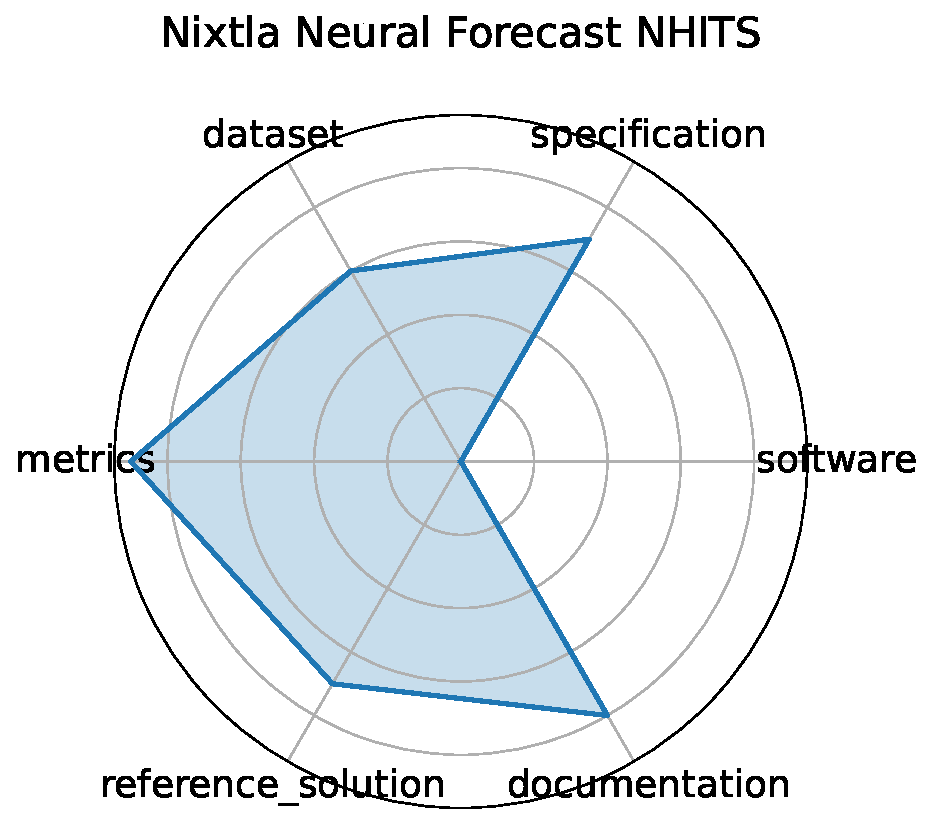
\includegraphics[width=0.2\textwidth]{nixtla_neural_forecast_nhits_radar.pdf}
}}
\clearpage